\documentclass[journal]{IEEEtran}
\usepackage[a5paper, margin=10mm, onecolumn]{geometry}
\usepackage{amsmath,amssymb,amsfonts,amsthm}
\usepackage{mathtools}
\usepackage{gvv-book}
\usepackage{gvv}
\usepackage{hyperref}

\begin{document}

\title{9.2.6}
\author{Puni Aditya - EE25BTECH11046}
\maketitle

\textbf{Question:}

Area of the region in the first quadrant enclosed by the x-axis, the line y = x and the circle $x^2 + y^2 = 32$ is \rule{2cm}{0.4pt}.

\textbf{Solution:}

Let the conic section be $g\brak{\vec{x}} = \vec{x}^\top\vec{V}\vec{x} + 2\vec{u}^\top\vec{x} + f = 0$.
Let the line be $\vec{x} = \vec{h} + \kappa\vec{m}$.
To find the points of intersection, we substitute the line equation into the conic equation.
\begin{align}
    g\brak{\vec{h}+\kappa\vec{m}} &= \brak{\vec{h}+\kappa\vec{m}}^\top\vec{V}\brak{\vec{h}+\kappa\vec{m}} + 2\vec{u}^\top\brak{\vec{h}+\kappa\vec{m}} + f = 0 \\
    &= \brak{\vec{h}^\top + \kappa\vec{m}^\top}\vec{V}\brak{\vec{h}+\kappa\vec{m}} + 2\vec{u}^\top\vec{h} + 2\kappa\vec{u}^\top\vec{m} + f = 0 \\
    &= \vec{h}^\top\vec{V}\vec{h} + 2\kappa\vec{m}^\top\vec{V}\vec{h} + \kappa^2\vec{m}^\top\vec{V}\vec{m} + 2\vec{u}^\top\vec{h} + 2\kappa\vec{u}^\top\vec{m} + f = 0 \\
    &= \brak{\vec{m}^\top\vec{V}\vec{m}}\kappa^2 + 2\brak{\vec{m}^\top\vec{V}\vec{h} + \vec{m}^\top\vec{u}}\kappa + \brak{\vec{h}^\top\vec{V}\vec{h} + 2\vec{u}^\top\vec{h} + f} = 0 \\
    &= \brak{\vec{m}^\top\vec{V}\vec{m}}\kappa^2 + 2\vec{m}^\top\brak{\vec{V}\vec{h} + \vec{u}}\kappa + g\brak{\vec{h}} = 0
\end{align}
This is a quadratic equation in $\kappa$.
\begin{align}
    \kappa_{1,2} = \frac{-2\vec{m}^\top\brak{\vec{V}\vec{h}+\vec{u}} \pm \sqrt{4\brak{\vec{m}^\top\brak{\vec{V}\vec{h}+\vec{u}}}^2 - 4\brak{\vec{m}^\top\vec{V}\vec{m}}g\brak{\vec{h}}}}{2\vec{m}^\top\vec{V}\vec{m}} \\
    \kappa_{1,2} = \frac{-\vec{m}^\top\brak{\vec{V}\vec{h}+\vec{u}} \pm \sqrt{\brak{\vec{m}^\top\brak{\vec{V}\vec{h}+\vec{u}}}^2 - \brak{\vec{m}^\top\vec{V}\vec{m}}g\brak{\vec{h}}}}{\vec{m}^\top\vec{V}\vec{m}} \label{eq:34}
\end{align}
Using \eqref{eq:34} to find the intersection points that define the boundaries of the area,
\begin{align*}
    \text{Circle: } x^2+y^2-32 = 0 \implies \vec{V}=\vec{I}, \vec{u}=\vec{0}, f=-32 \\
    \text{Lines: } \vec{x} = \kappa\myvec{1 \\ 0},\text{ so } \vec{h_1}=\vec{0}, \vec{m_1}=\myvec{1 \\ 0}\text{ and } \vec{x} = \kappa\myvec{1 \\ 1},\text{ so } \vec{h_2}=\vec{0}, \vec{m_2}=\myvec{1 \\ 1}
\end{align*}
\begin{align}
    g\brak{\vec{h_1}} &= g\brak{\vec{0}} = -32 \\
    \vec{m_1}^\top\vec{V}\vec{m_1} &= \myvec{1&0}\vec{I}\myvec{1\\0} = 1 \\
    \vec{m_1}^\top\brak{\vec{V}\vec{h_1}+\vec{u}} &= \myvec{1&0}\brak{\vec{I}\vec{0}+\vec{0}} = 0
\end{align}
\begin{align}
    \kappa = \frac{0 \pm \sqrt{0^2 - \brak{1}\brak{-32}}}{1} = \pm\frac{\sqrt{32}}{1} = \pm 4\sqrt{2}
\end{align}
\begin{align}
    g\brak{\vec{h_2}} &= g\brak{\vec{0}} = -32 \\
    \vec{m_2}^\top\vec{V}\vec{m_2} &= \myvec{1&1}\vec{I}\myvec{1\\1} = 2 \\
    \vec{m_2}^\top\brak{\vec{V}\vec{h_2}+\vec{u}} &= \myvec{1&1}\brak{\vec{I}\vec{0}+\vec{0}} = 0
\end{align}
\begin{align}
    \kappa = \frac{0 \pm \sqrt{0^2 - \brak{2}\brak{-32}}}{2} = \pm\frac{\sqrt{64}}{2} = \pm 4
\end{align}
The intersection points are
\begin{align}
    \vec{x_i} = \kappa \vec{m_i}
\end{align}
In the first quadrant, the intersection points defining the region are:
\begin{align}
    \vec{x_1} &= \myvec{4\sqrt{2} \\ 0}, \text{ } \vec{x_2} = \myvec{4 \\ 4}
\end{align}
The area is the sum of two integrals, split at the x-coordinate of $\vec{x_2}$.
\begin{align}
    A &= \int_{0}^{4} x \, dx + \int_{4}^{4\sqrt{2}} \sqrt{32-x^2} \, dx \\
    &= \sbrak{ \frac{x^2}{2} }_{0}^{4} + \sbrak{ \frac{x}{2}\sqrt{32-x^2} + 16\sin^{-1}\brak{\frac{x}{4\sqrt{2}}} }_{4}^{4\sqrt{2}} \\
    &= \frac{16}{2} + \sbrak{ 0 + 16\sin^{-1}\brak{1} } - \sbrak{ \frac{4}{2}\sqrt{16} + 16\sin^{-1}\brak{\frac{1}{\sqrt{2}}} } \\
    &= 8 + 16\brak{\frac{\pi}{2}} - \sbrak{ 8 + 16\brak{\frac{\pi}{4}} } \\
    &= 8 + 8\pi - 8 - 4\pi = 4\pi
\end{align}

\begin{figure}[h!]
	\centering
	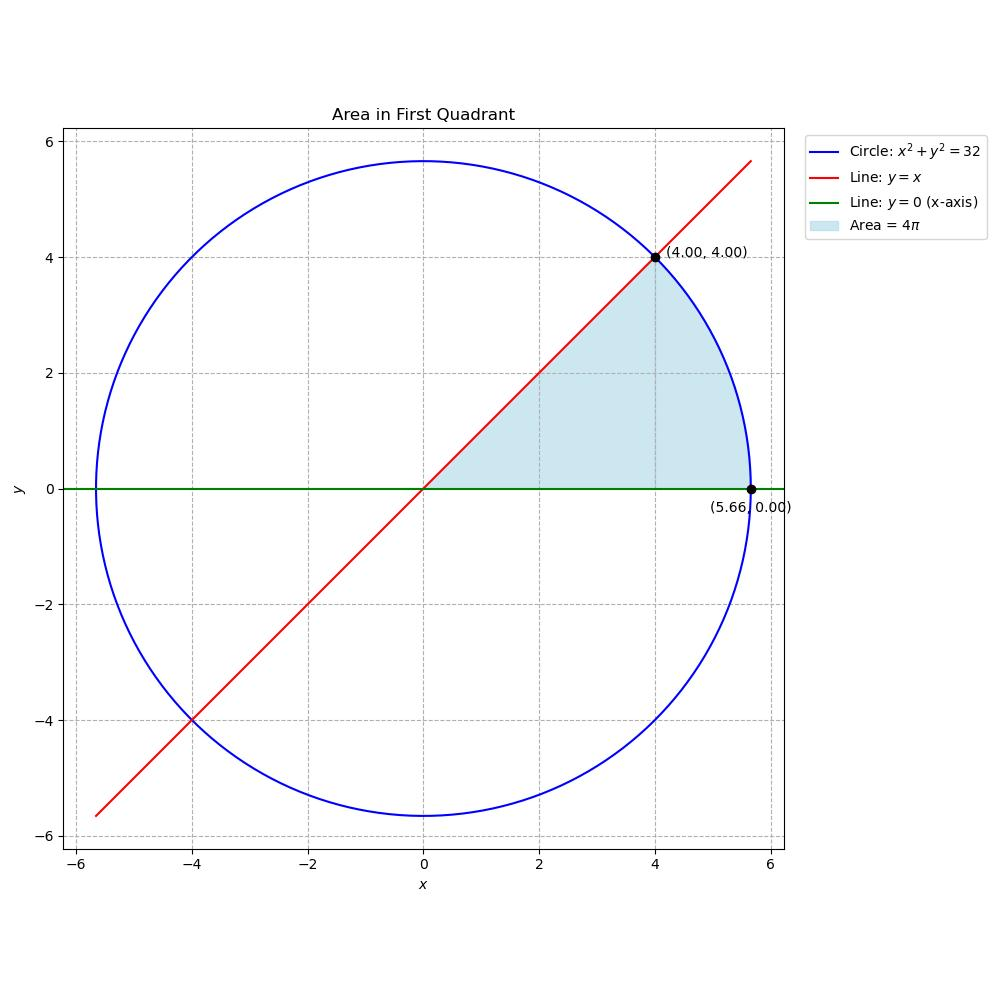
\includegraphics[width=\columnwidth]{figs/plot_c.jpg}
	\caption*{Plot}
	\label{fig:fig}
\end{figure}

\end{document}
